% Foundation-model study manuscript. Numbers are macros from generated/values.tex
% (foundation_models/scripts/make_paper.py). Build: make fm-docs
\documentclass[10pt]{article}
\usepackage[a4paper, margin=22mm, top=24mm, bottom=26mm]{geometry}
\usepackage{fontspec}
\usepackage{amsmath, amssymb}
\usepackage{graphicx}
\usepackage{booktabs, tabularx}
\usepackage{xcolor}
\usepackage[font=small, labelfont=bf, labelsep=period, justification=justified,
            singlelinecheck=false]{caption}
\usepackage{titlesec}
\usepackage{enumitem}
\usepackage{microtype}
\usepackage[hidelinks]{hyperref}
\usepackage{fancyhdr}
\usepackage{float}

\definecolor{ink}{HTML}{161B1F}
\definecolor{cobalt}{HTML}{2457D6}
\definecolor{vermilion}{HTML}{E33D3F}
\definecolor{rule}{HTML}{D9DDE0}
\definecolor{subtle}{HTML}{5B6670}
\color{ink}
\hypersetup{colorlinks=true, linkcolor=cobalt, citecolor=cobalt, urlcolor=cobalt}

\setmainfont{IBMPlexSans}[Path=../../.cache/fonts/, Extension=.ttf, UprightFont=*-Regular,
  BoldFont=*-SemiBold, ItalicFont=*-Italic, BoldItalicFont=*-SemiBold]
\setsansfont{IBMPlexSans}[Path=../../.cache/fonts/, Extension=.ttf, UprightFont=*-Regular,
  BoldFont=*-SemiBold, ItalicFont=*-Italic, BoldItalicFont=*-SemiBold]
\setmonofont{IBMPlexMono}[Path=../../.cache/fonts/, Extension=.ttf, UprightFont=*-Regular,
  BoldFont=*-Medium, Scale=0.9]
\newfontfamily\editorial{Fraunces}[Path=../../assets/fonts/, Extension=.ttf,
  UprightFont=*-SemiBold, BoldFont=*-SemiBold]
\newfontfamily\editoriallight{Fraunces}[Path=../../assets/fonts/, Extension=.ttf,
  UprightFont=*-Regular]

\usepackage[italic]{mathastext}
\linespread{1.12}
\setlength{\emergencystretch}{2em}
\setlength{\parindent}{0pt}
\setlength{\parskip}{0.55em}
\titleformat{\section}{\editorial\Large\color{ink}}{\thesection}{0.7em}{}
\titleformat{\subsection}{\editorial\large\color{ink}}{\thesubsection}{0.7em}{}
\titleformat{\paragraph}[runin]{\bfseries}{}{}{}[.]
\titlespacing*{\section}{0pt}{1.6em}{0.5em}
\titlespacing*{\subsection}{0pt}{1.2em}{0.35em}
\setlist{itemsep=0.15em, topsep=0.2em}
\captionsetup{labelfont={bf,color=ink}, font={small,color=ink}}
\renewcommand{\arraystretch}{1.15}
\newcommand{\figref}[1]{Fig.~\ref{#1}}

\pagestyle{fancy}
\fancyhf{}
\renewcommand{\headrulewidth}{0pt}
\fancyfoot[L]{\footnotesize\color{subtle}\texttt{Tabular foundation models on a small biological dataset}}
\fancyfoot[R]{\footnotesize\color{subtle}\thepage}

% Generated by foundation_models/scripts/make_paper.py -- do not edit.
\newcommand{\BABest}{0.660}
\newcommand{\BADummy}{0.125}
\newcommand{\BAElasticNet}{0.619}
\newcommand{\BAGradBoost}{0.550}
\newcommand{\BAKumo}{0.818}
\newcommand{\BALogistic}{0.660}
\newcommand{\BARandomForest}{0.536}
\newcommand{\BASDDummy}{0.000}
\newcommand{\BASDElasticNet}{0.018}
\newcommand{\BASDGradBoost}{0.027}
\newcommand{\BASDKumo}{0.017}
\newcommand{\BASDLogistic}{0.029}
\newcommand{\BASDRandomForest}{0.034}
\newcommand{\BASDSVM}{0.030}
\newcommand{\BASDTabpfn}{0.018}
\newcommand{\BASVM}{0.576}
\newcommand{\BATabpfn}{0.744}
\newcommand{\BestBaseline}{Logistic (L2)}
\newcommand{\BestBaselineLL}{Logistic (L2)}
\newcommand{\BrierDummy}{0.88}
\newcommand{\BrierElasticNet}{0.54}
\newcommand{\BrierGradBoost}{0.71}
\newcommand{\BrierKumo}{0.29}
\newcommand{\BrierLogistic}{0.47}
\newcommand{\BrierRandomForest}{0.62}
\newcommand{\BrierSVM}{0.64}
\newcommand{\BrierTabpfn}{0.38}
\newcommand{\DocAuthor}{Noushin}
\newcommand{\ECEDummy}{0.00}
\newcommand{\ECEElasticNet}{0.18}
\newcommand{\ECEGradBoost}{0.30}
\newcommand{\ECEKumo}{0.07}
\newcommand{\ECELogistic}{0.09}
\newcommand{\ECERandomForest}{0.17}
\newcommand{\ECESVM}{0.25}
\newcommand{\ECETabpfn}{0.12}
\newcommand{\FactorCondKumo}{1.00}
\newcommand{\FactorCondLogistic}{1.00}
\newcommand{\FactorCondTabpfn}{1.00}
\newcommand{\FactorGenoKumo}{0.91}
\newcommand{\FactorGenoLogistic}{0.86}
\newcommand{\FactorGenoTabpfn}{0.91}
\newcommand{\FactorTreatKumo}{0.87}
\newcommand{\FactorTreatLogistic}{0.73}
\newcommand{\FactorTreatTabpfn}{0.67}
\newcommand{\HfourA}{supported}
\newcommand{\HfourB}{supported}
\newcommand{\HfourC}{supported}
\newcommand{\HoneKumo}{supported}
\newcommand{\HoneKumoBeaten}{6}
\newcommand{\HoneKumoCI}{+0.026 to +0.274}
\newcommand{\HoneKumoDiff}{+0.150}
\newcommand{\HoneKumoP}{0.020}
\newcommand{\HoneTabpfn}{not supported}
\newcommand{\HoneTabpfnBeaten}{2}
\newcommand{\HoneTabpfnCI}{-0.053 to +0.198}
\newcommand{\HoneTabpfnDiff}{+0.072}
\newcommand{\HoneTabpfnP}{0.277}
\newcommand{\HthreeKumo}{not supported}
\newcommand{\HthreeKumoCI}{-0.160 to -0.051}
\newcommand{\HthreeKumoDiff}{-0.104}
\newcommand{\HthreeKumoLarge}{+0.153}
\newcommand{\HthreeKumoSmall}{+0.049}
\newcommand{\HthreeTabpfn}{not supported}
\newcommand{\HthreeTabpfnCI}{-0.119 to +0.003}
\newcommand{\HthreeTabpfnDiff}{-0.058}
\newcommand{\HthreeTabpfnLarge}{+0.087}
\newcommand{\HthreeTabpfnSmall}{+0.030}
\newcommand{\HtwoKumo}{supported}
\newcommand{\HtwoKumoBeaten}{6}
\newcommand{\HtwoKumoCI}{+0.220 to +1.105}
\newcommand{\HtwoKumoDiff}{+0.662}
\newcommand{\HtwoKumoP}{0.005}
\newcommand{\HtwoTabpfn}{not supported}
\newcommand{\HtwoTabpfnBeaten}{4}
\newcommand{\HtwoTabpfnCI}{-0.047 to +0.976}
\newcommand{\HtwoTabpfnDiff}{+0.464}
\newcommand{\HtwoTabpfnP}{0.073}
\newcommand{\LCsixKumo}{0.77}
\newcommand{\LCsixLogistic}{0.62}
\newcommand{\LCsixRandomForest}{0.55}
\newcommand{\LCsixSVM}{0.50}
\newcommand{\LCsixTabpfn}{0.70}
\newcommand{\LCtwoKumo}{0.46}
\newcommand{\LCtwoLogistic}{0.41}
\newcommand{\LCtwoRandomForest}{0.42}
\newcommand{\LCtwoSVM}{0.34}
\newcommand{\LCtwoTabpfn}{0.44}
\newcommand{\LLBest}{1.23}
\newcommand{\LLDummy}{2.09}
\newcommand{\LLElasticNet}{1.36}
\newcommand{\LLGradBoost}{2.04}
\newcommand{\LLKumo}{0.56}
\newcommand{\LLLogistic}{1.23}
\newcommand{\LLRandomForest}{1.25}
\newcommand{\LLSVM}{1.33}
\newcommand{\LLTabpfn}{0.76}
\newcommand{\LeakMiceKumo}{0.765}
\newcommand{\LeakMiceLogistic}{0.712}
\newcommand{\LeakMiceRandomForest}{0.619}
\newcommand{\LeakMiceTabpfn}{0.653}
\newcommand{\LeakRowsKumo}{1.000}
\newcommand{\LeakRowsLogistic}{0.994}
\newcommand{\LeakRowsRandomForest}{0.990}
\newcommand{\LeakRowsTabpfn}{0.999}
\newcommand{\MemKumoDrop}{+0.003}
\newcommand{\MemKumoObf}{0.814}
\newcommand{\MemKumoOrig}{0.818}
\newcommand{\MemTabpfnDrop}{+0.006}
\newcommand{\MemTabpfnObf}{0.738}
\newcommand{\MemTabpfnOrig}{0.744}
\newcommand{\PermMax}{0.139}
\newcommand{\PermMin}{0.121}
\newcommand{\SecDummy}{0.00}
\newcommand{\SecElasticNet}{0.96}
\newcommand{\SecGradBoost}{0.95}
\newcommand{\SecKumo}{1.01}
\newcommand{\SecLogistic}{0.01}
\newcommand{\SecRandomForest}{0.30}
\newcommand{\SecSVM}{0.06}
\newcommand{\SecTabpfn}{1.39}
\newcommand{\SklearnVersion}{1.6.1}
\newcommand{\TabpfnVersion}{2.2.1}
\newcommand{\TorchVersion}{2.15.0}

\hypersetup{pdftitle={Tabular foundation models on a small biological dataset}, pdfauthor={\DocAuthor}}

\begin{document}

\begin{flushleft}
{\color{subtle}\small\texttt{RESEARCH ARTICLE \textbullet{} PRE-SPECIFIED COMPARISON}}\par\vspace{0.6em}
{\editorial\fontsize{21}{25}\selectfont Kumo leads the tested models on 72 mice; a later
matched-holdout analysis examines sample efficiency\par}
\vspace{0.7em}
{\editoriallight\large A controlled comparison of TabPFN and Kumo on cortical protein profiles
from a mouse model of Down syndrome\par}
\vspace{0.9em}
{\small\color{subtle}Questions, hypotheses and decision rules were fixed and committed before
the experiments were run. Every number is regenerated from the raw data.\par}
\end{flushleft}
\vspace{0.4em}
{\color{rule}\rule{\linewidth}{0.6pt}}

\begin{abstract}
\noindent\textbf{Problem.} Tabular foundation models (TFMs) are pretrained on very large
collections of tables and predict new tables \emph{in context}, without task-specific training.
They are widely described as strongest on small datasets, the usual situation in biology.
Testing that claim on real biological data is hard: there are few independent samples,
differences between models are small relative to resampling noise, and public datasets may
already be in a model's pretraining data.
\textbf{Approach.} On the UCI Mice Protein Expression data (72 mice, 77 cortical proteins,
eight experimental groups) we compared TabPFN v2 and Kumo Tabular Small with six conventional
baselines on identical held-out mice. We pre-specified four questions: accuracy (RQ1),
probabilistic prediction (RQ2), data efficiency (RQ3) and validity (RQ4), with corrected paired tests,
learning curves and three control experiments.
\textbf{Findings.} In the original comparison Kumo reached \BAKumo{} eight-group balanced
accuracy and led the initially tested baselines (best: \BestBaseline, \BABest). TabPFN
reached \BATabpfn{}. Kumo had the lowest observed log loss (\LLKumo{} vs \LLBest),
which does not establish superior calibration. A later, exploratory nested search moved
logistic regression to 0.675; Kumo's corrected paired-fold comparison with this tuned
baseline had an unadjusted $p=0.072$ and an approximate interval crossing zero. A
post hoc fixed-holdout curve with five subset draws per split found a mean Kumo-minus-logistic
gap of 0.077 with 16 labeled mice and 0.122 with 48, but the change varied across draws.
Shuffled labels gave near-chance accuracy and random row splits inflated scores.
Feature obfuscation cannot establish absence of checkpoint contamination.
\textbf{Conclusion.} On this cohort Kumo led the tested configurations, but superiority
over a tuned conventional model and generalization to new cohorts are not established.
The original protocol and post hoc amendments are distinguished in the repository.
\end{abstract}

\begin{figure}[h]
\centering
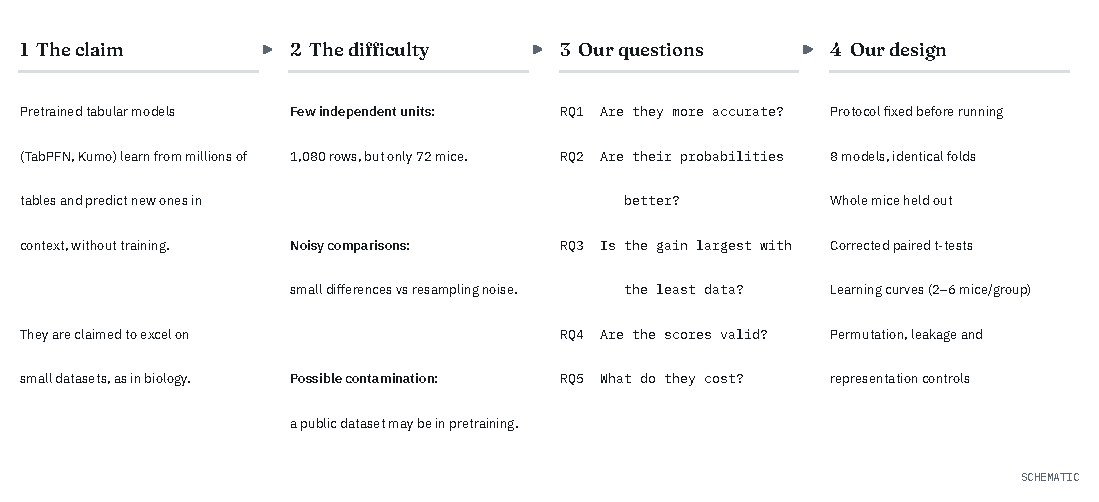
\includegraphics[width=\linewidth]{../results/figures/fig0_overview.pdf}
\caption{\textbf{Study at a glance.} The claim being tested, why testing it is difficult, our
questions and design. Schematic.}
\label{fig:overview}
\end{figure}

\section{Introduction}

\paragraph{Background} Tabular data, tables of samples and measured variables, are the most
common data type in biology and medicine. For decades the strongest methods have been
regularised linear models and tree ensembles \cite{grinsztajn2022}. TFMs take a different
approach: a large neural network is pretrained on millions of tables, synthetic or real, and
then predicts the labels of a new table by reading its training rows as context, with no
gradient-based training \cite{hollmann2025}. Because the model brings a learned prior about
how tables behave, it is often expected to shine where data are scarce.

\paragraph{The problem} Biological studies are typically small, so this claim matters, but it
is hard to test fairly. Three difficulties arise in the dataset used here.
\begin{enumerate}[label=\arabic*., leftmargin=1.6em]
\item \textbf{Few independent units.} The table has 1{,}080 rows but only 72 mice; each mouse
  was measured 15 times. Splitting rows at random leaks each mouse into training and test data
  \cite{lazic2010, kaufman2012}.
\item \textbf{Noisy comparisons.} With 72 mice, model differences are small relative to the
  variation between cross-validation splits, and naive paired tests are over-confident
  because the splits share training data \cite{nadeau2003}.
\item \textbf{Possible contamination.} The dataset is public, so a TFM may have seen it during
  pretraining.
\end{enumerate}

\paragraph{Our questions} We therefore ask four questions, each with a hypothesis fixed before
any experiment was run:
\begin{enumerate}[label=\textbf{RQ\arabic*.}, leftmargin=2.8em]
\item \textbf{Accuracy.} Are TFMs more accurate than the selected conventional models?
  (H1: each TFM beats every baseline.)
\item \textbf{Calibration.} Are their predicted probabilities better? (H2: lower log loss than
  every baseline.)
\item \textbf{Data efficiency.} Is their advantage largest when data are scarcest? (H3: a larger
  lead over logistic regression with 2 than with 6 training mice per group.)
\item \textbf{Validity.} Are the scores trustworthy? (H4: chance accuracy with shuffled labels;
  inflation under row-level leakage; no reliance on dataset identity.)
\end{enumerate}
We also report computational cost (RQ5) and, as exploratory analyses, per-group errors and
accuracy for each experimental factor. Box~1 defines the main terms.

\begin{figure}[!htb]
\noindent\fcolorbox{rule}{white}{\begin{minipage}{0.97\linewidth}
\small\vspace{0.3em}
{\editorial\normalsize Box 1 \textbullet{} Key concepts}
\begin{description}[leftmargin=0pt, itemsep=0.25em, font=\bfseries]
\item[Tabular foundation model.] A network pretrained on many tables that predicts a new table's
  labels from its training rows, read as context (\emph{in-context learning}).
\item[Balanced accuracy (BA).] The average, over groups, of the share of each group predicted
  correctly. With eight groups, chance is 0.125.
\item[Log loss.] The average of $-\log$ of the probability assigned to the true group; low only
  when the model is confident \emph{and} right.
\item[Calibration.] Whether predictions made with confidence $c$ are correct a fraction $c$ of
  the time; summarised by the expected calibration error (ECE).
\item[Corrected paired $t$-test.] Compares two models fold by fold, inflating the variance to
  account for folds that share training data \cite{nadeau2003, bouckaert2004}.
\item[Holm correction.] Adjusts $p$-values when one model is compared with several others
  \cite{holm1979}.
\end{description}
\end{minipage}}
\end{figure}

\section{Data and design}

The UCI Mice Protein Expression dataset \cite{uci2015} records 77 proteins and protein
modifications in the cortex of 72 male mice: control or Ts65Dn (a Down-syndrome model), trained
with or without the opportunity to learn a context--shock association, and injected with
memantine or saline \cite{ahmed2015, higuera2015}. These three factors define eight groups of
7--10 mice. Each mouse was measured 15 times (three replicates of a five-point dilution series);
we average these into one profile per mouse, so every analysis treats the mouse as the unit.
The primary task is predicting a held-out mouse's group (8 classes); predicting each factor
separately is secondary.

Eight models were compared (Table~\ref{tab:performance}): a class-prior baseline; L2 logistic
regression; elastic net, RBF support-vector machine and histogram gradient boosting, each tuned
by three-fold inner cross-validation; a random forest; and the two TFMs, TabPFN v2 and Kumo
Tabular Small, used without tuning and with four inference estimators each. All models were evaluated on five repeats of five-fold
cross-validation stratified by group, with \emph{identical folds for every model}.

\section{Results}

Table~\ref{tab:hypotheses} summarises the verdict on every pre-specified hypothesis; the sections
below explain each one.

\begin{table}[h]
\centering
\caption{\textbf{Verdicts on the pre-specified hypotheses.} Rules are stated in Methods and were
fixed before the experiments. H1, H2 and H4c were written knowing an earlier benchmark on the
same data, so they are informed rather than blind; H3, H4a and H4b were blind.}
\label{tab:hypotheses}
\small
\begin{tabularx}{\linewidth}{lXl}
\toprule
Hypothesis & Statement (fixed in advance) & Verdict \\
\midrule
H1 & TFMs more accurate than every baseline & TabPFN: not supported; Kumo: supported \\
H2 & TFMs have lower log loss than every baseline & TabPFN: not supported; Kumo: supported \\
H3 & TFM advantage larger at 2 than at 6 mice per group & TabPFN: not supported; Kumo: not supported \\
H4a & All models at chance with shuffled labels & supported \\
H4b & All models inflated by row-level leakage & supported \\
H4c & No reliance on dataset identity & supported \\
\bottomrule
\end{tabularx}

\end{table}

\subsection{RQ1. Kumo is more accurate than every baseline; TabPFN is not}
\textit{Question: are TFMs more accurate than tuned conventional models? Answer: Kumo yes, by a
margin that survives correction; TabPFN's lead over the best baseline is within noise.}

\begin{figure}[t]
\centering
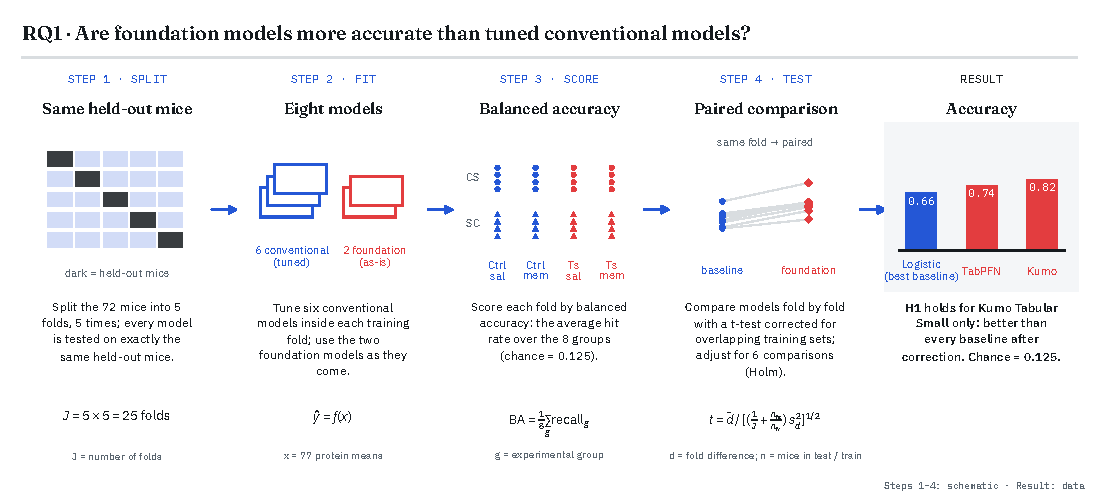
\includegraphics[width=\linewidth]{../results/figures/workflows/wf_rq1_accuracy.pdf}
\caption{\textbf{Workflow for RQ1.} Each step shows its defining equation; the result panel
shows the measured accuracies. Steps are schematic.}
\end{figure}

Kumo reached a balanced accuracy of \BAKumo{} and TabPFN \BATabpfn, against \BABest{} for the
best conventional model, \BestBaseline{} (\figref{fig:accuracy}a; Table~\ref{tab:performance}).
Notably, the simplest baseline was the strongest: tuned elastic net (\BAElasticNet), SVM
(\BASVM), gradient boosting (\BAGradBoost) and random forest (\BARandomForest) all scored lower.

Under the corrected test, Kumo beat all \HoneKumoBeaten{} comparators, including
\BestBaseline{} by \HoneKumoDiff{} (95\% CI \HoneKumoCI; Holm-adjusted $p = \HoneKumoP$;
\figref{fig:accuracy}c). TabPFN beat the class prior and the random forest, but its advantage
over \BestBaseline{} (\HoneTabpfnDiff; CI \HoneTabpfnCI; $p = \HoneTabpfnP$) could not be
distinguished from zero (\figref{fig:accuracy}b). H1 is therefore \HoneKumo{} for Kumo and
\HoneTabpfn{} for TabPFN. Full test results are in Table~\ref{tab:tests}.

\begin{figure}[t]
\centering
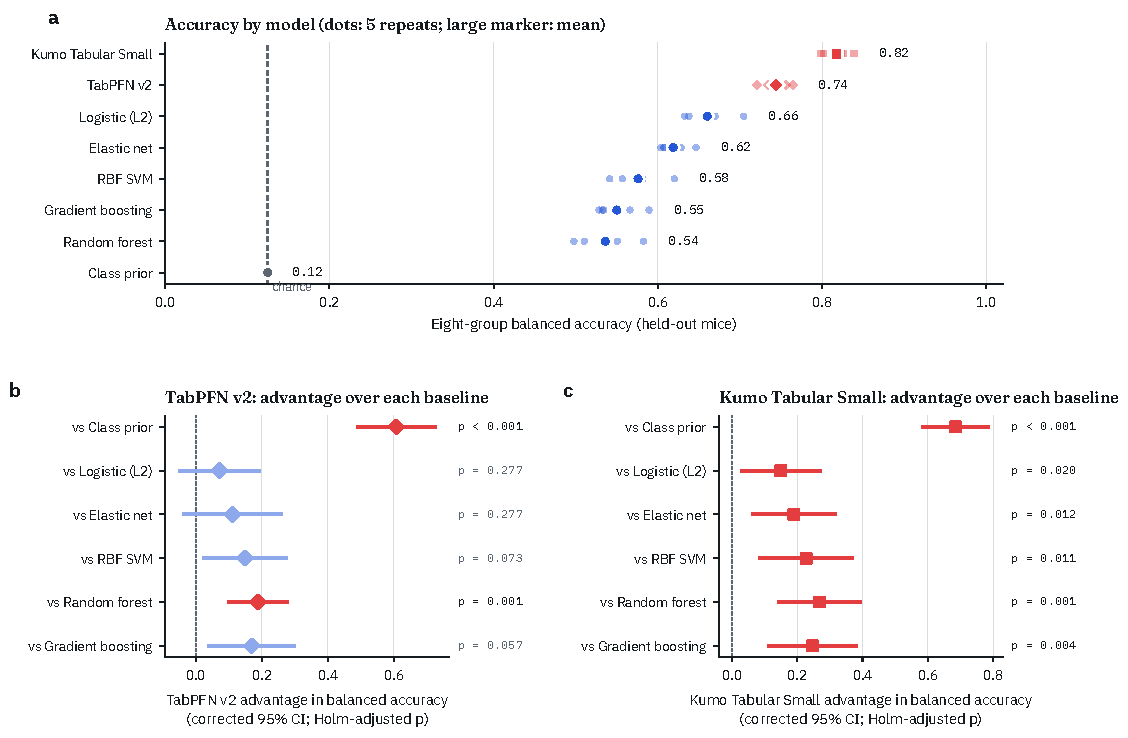
\includegraphics[width=\linewidth]{../results/figures/fig1_accuracy.pdf}
\caption{\textbf{Accuracy.} \textbf{a}, Eight-group balanced accuracy for held-out mice: small
markers are the five repeats; large markers their mean. \textbf{b, c}, Paired advantage of each
TFM over each baseline, with 95\% intervals from the Nadeau--Bengio corrected $t$-test and
Holm-adjusted $p$-values; coloured intervals are significant improvements.}
\label{fig:accuracy}
\end{figure}

\subsection{RQ2. Kumo has the lowest log loss among tested models}
\textit{Question: are TFM probabilities better? Answer: Kumo's are better than every baseline's;
TabPFN's are better than most but not all.}

\begin{figure}[t]
\centering
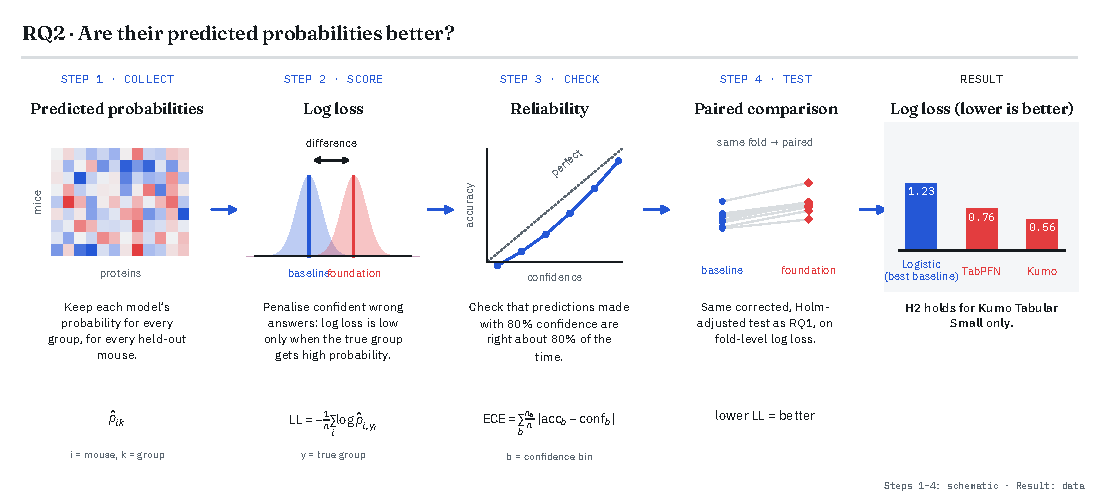
\includegraphics[width=\linewidth]{../results/figures/workflows/wf_rq2_calibration.pdf}
\caption{\textbf{Workflow for RQ2.} Schematic steps; the result panel shows measured log loss.}
\end{figure}

Log loss was \LLKumo{} for Kumo and \LLTabpfn{} for TabPFN, against \LLBest{} for the best
baseline (\BestBaselineLL) and 2.08 for a uniform guess (\figref{fig:calibration}a). Kumo
improved on every baseline (H2 \HtwoKumo; vs \BestBaselineLL{} \HtwoKumoDiff, $p = \HtwoKumoP$).
TabPFN improved on four of six, but not on logistic regression or elastic net after correction
(H2 \HtwoTabpfn). Expected calibration error was \ECEKumo{} for Kumo, \ECETabpfn{} for TabPFN and
\ECELogistic{} for logistic regression. These descriptive estimates reuse the same mice across
repeats; lower log loss does not, by itself, establish superior calibration.

\begin{figure}[t]
\centering
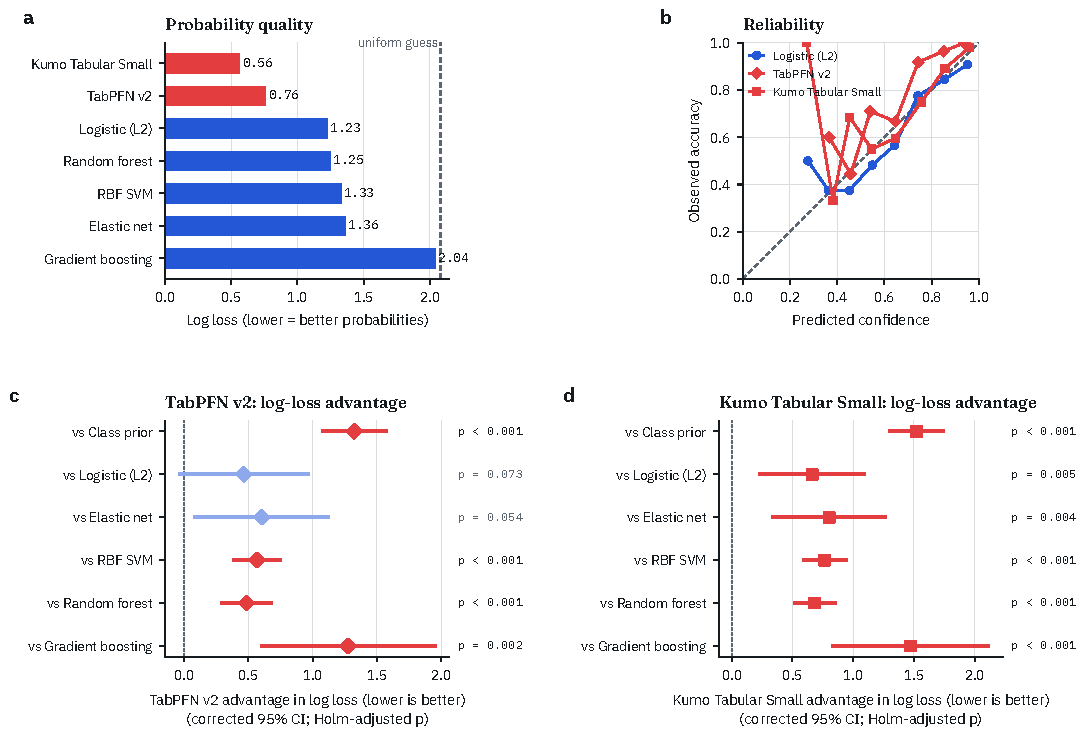
\includegraphics[width=\linewidth]{../results/figures/fig2_calibration.pdf}
\caption{\textbf{Calibration.} \textbf{a}, Log loss (lower is better); dashed line: uniform
guess. \textbf{b}, Reliability diagram (pooled out-of-fold predictions; diagonal = perfect
calibration). \textbf{c, d}, Paired log-loss advantage of each TFM over each baseline
(corrected 95\% CI; Holm-adjusted $p$).}
\label{fig:calibration}
\end{figure}

\subsection{RQ3. Original learning curves suggested a growing advantage}
\textit{Question: is the TFM advantage largest when data are scarcest? Answer: no. For both
models the lead over logistic regression is smallest with 2 mice per group and grows with more
data.}

\begin{figure}[t]
\centering
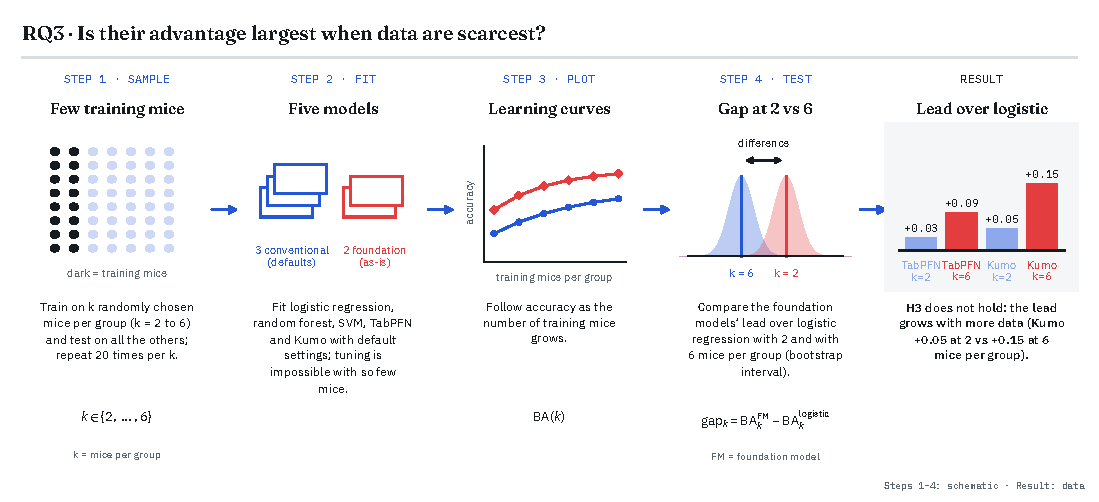
\includegraphics[width=\linewidth]{../results/figures/workflows/wf_rq3_learning.pdf}
\caption{\textbf{Workflow for RQ3.} Schematic steps; the result panel shows the measured lead
over logistic regression with 2 and 6 training mice per group.}
\end{figure}

With 2 training mice per group (16 mice in total), all models were close: Kumo \LCtwoKumo,
TabPFN \LCtwoTabpfn, logistic regression \LCtwoLogistic. With 6 per group, Kumo reached
\LCsixKumo{} and TabPFN \LCsixTabpfn, against \LCsixLogistic{} for logistic regression
(\figref{fig:learning}a). The TFM lead over logistic regression therefore grew, from
\HthreeTabpfnSmall{} to \HthreeTabpfnLarge{} for TabPFN and from \HthreeKumoSmall{} to
\HthreeKumoLarge{} for Kumo (\figref{fig:learning}b). The pre-specified difference
(gap at 2 minus gap at 6) was \HthreeKumoDiff{} for Kumo (95\% CI \HthreeKumoCI) and
\HthreeTabpfnDiff{} for TabPFN (CI \HthreeTabpfnCI), so H3 is \HthreeKumo under the original
decision rule. However, test mice change with training size, and repeated draws reuse the same
animals. The interval does not measure uncertainty across biological cohorts. The repository
contains a later, post hoc matched-holdout extension that addresses test-set composition.

\begin{figure}[t]
\centering
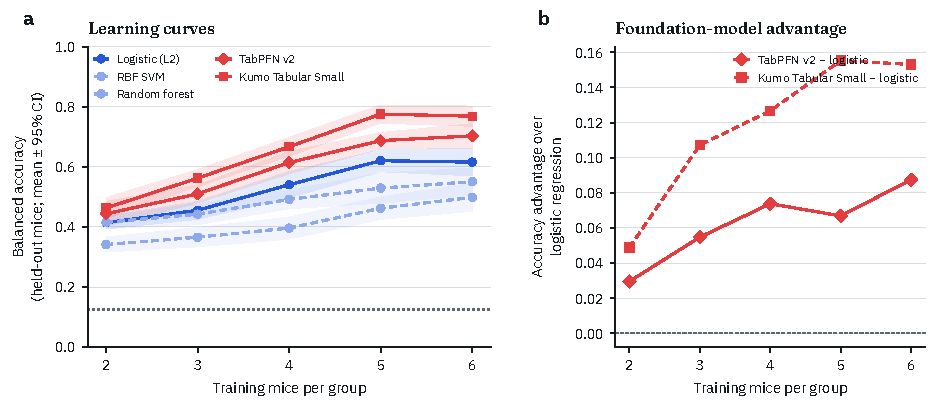
\includegraphics[width=\linewidth]{../results/figures/fig3_learning_curves.pdf}
\caption{\textbf{Learning curves.} \textbf{a}, Balanced accuracy on held-out mice as the number
of training mice per group grows (mean and interval over 20 draws from the same cohort; this is
not a biological-population confidence interval).
\textbf{b}, Advantage of each TFM over logistic regression.}
\label{fig:learning}
\end{figure}

\subsection{RQ4. All three validity controls behave as specified}
\textit{Question: can the scores be trusted? Answer: yes, as far as these controls can tell.}

\begin{figure}[t]
\centering
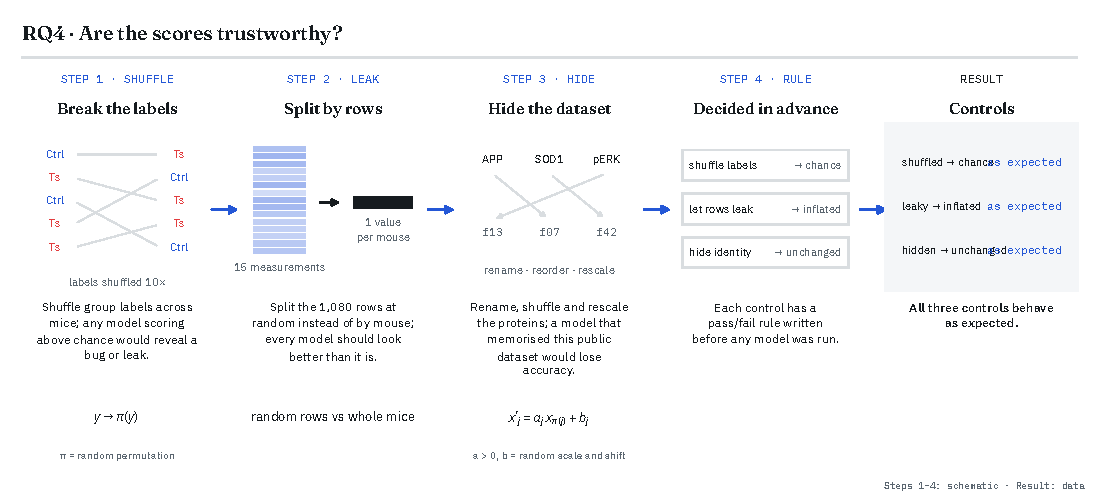
\includegraphics[width=\linewidth]{../results/figures/workflows/wf_rq4_validity.pdf}
\caption{\textbf{Workflow for RQ4.} Three controls, each with a rule fixed in advance.}
\end{figure}

\paragraph{Shuffled labels} With labels permuted across mice, every model's mean balanced
accuracy lay between \PermMin{} and \PermMax{}, around the chance level of 0.125
(\figref{fig:validity}a; H4a \HfourA). No model, including the TFMs, extracts signal where none
exists, which rules out gross leakage in the pipeline.

\paragraph{Row-level leakage} Splitting the 1{,}080 rows at random instead of by mouse inflated
every model to near-perfect accuracy (logistic regression \LeakRowsLogistic, TabPFN
\LeakRowsTabpfn, Kumo \LeakRowsKumo), compared with \LeakMiceLogistic, \LeakMiceTabpfn{} and
\LeakMiceKumo{} when whole mice were held out (\figref{fig:validity}b; H4b \HfourB). Foundation
models are as vulnerable to this mistake as conventional ones.

\paragraph{Representation robustness} After renaming, shuffling and rescaling every protein, accuracy was
essentially unchanged: TabPFN \MemTabpfnOrig{} to \MemTabpfnObf, Kumo \MemKumoOrig{} to
\MemKumoObf{} (\figref{fig:validity}c; original H4c \HfourC). This checks sensitivity to
the chosen representation; it cannot establish absence of pretraining contamination.

\begin{figure}[t]
\centering
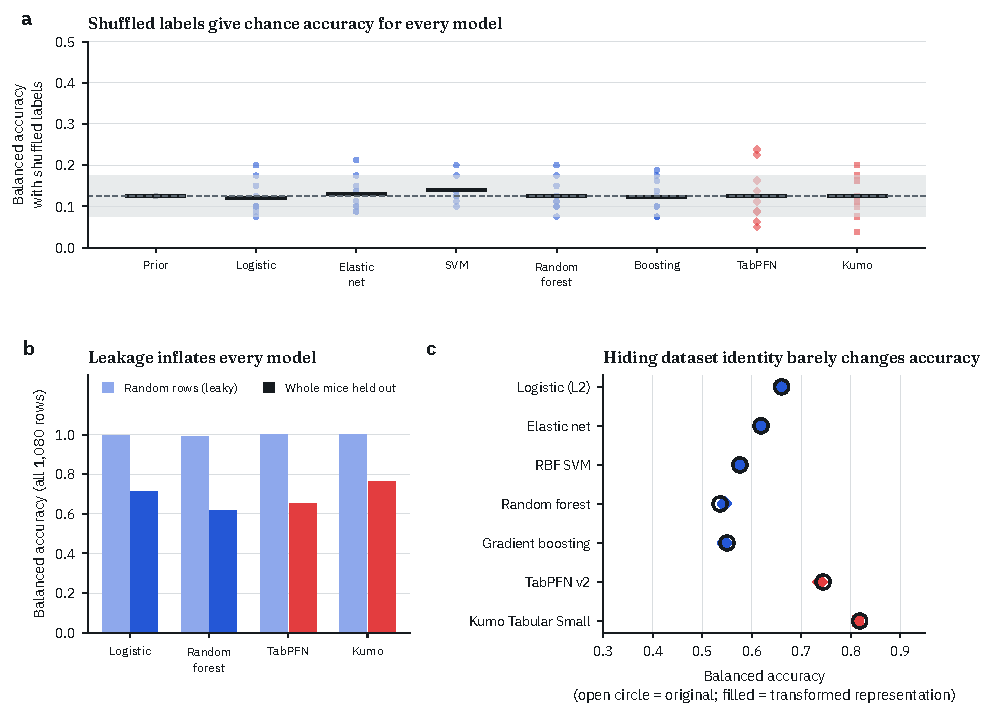
\includegraphics[width=\linewidth]{../results/figures/fig4_validity.pdf}
\caption{\textbf{Validity controls.} \textbf{a}, Balanced accuracy with shuffled labels
(10 permutations; band: chance $\pm$ 0.05). \textbf{b}, Accuracy on all 1{,}080 rows with a
random-row split (leaky) or with whole mice held out. \textbf{c}, Accuracy on the original data
(open circles) and after hiding the dataset's identity (filled markers; mean of three keys).}
\label{fig:validity}
\end{figure}

\subsection{Cost and exploratory analyses}
Fitting and predicting one fold took a median of \SecTabpfn{} s for TabPFN and \SecKumo{} s for
Kumo on a laptop CPU, against \SecLogistic{} s for logistic regression (\figref{fig:cost}a).
Errors concentrated in the control context--shock groups for all models
(\figref{fig:cost}b). For single factors (exploratory), all models identified conditioning
almost perfectly; for genotype, TFMs reached \FactorGenoKumo{} (Kumo) and \FactorGenoTabpfn{}
(TabPFN) against \FactorGenoLogistic{} for logistic regression; for treatment, Kumo reached
\FactorTreatKumo{}, TabPFN \FactorTreatTabpfn{} and logistic regression \FactorTreatLogistic.

\begin{figure}[t]
\centering
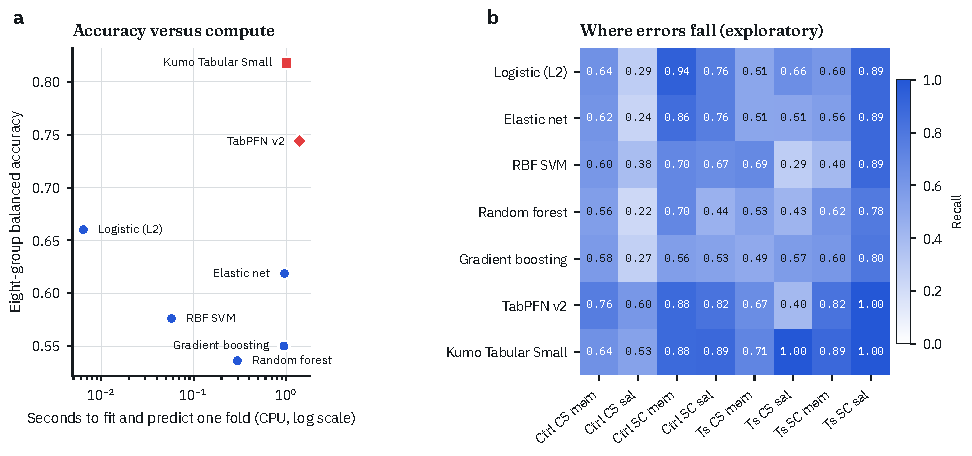
\includegraphics[width=\linewidth]{../results/figures/fig5_cost_errors.pdf}
\caption{\textbf{Cost and errors.} \textbf{a}, Accuracy against computing time per fold (log
scale). \textbf{b}, Recall for each experimental group (pooled out-of-fold predictions;
exploratory).}
\label{fig:cost}
\end{figure}

\begin{table}[t]
\centering
\caption{\textbf{Performance of every model.} Mean over five repeats of pooled out-of-fold
predictions; SD across repeats; s/fold: median seconds to fit and predict one fold (CPU).}
\label{tab:performance}
\small
\begin{tabular}{lrrrrrr}
\toprule
Model & BA & (SD) & Log loss & Brier & ECE & s/fold \\
\midrule
Class prior & 0.125 & 0.000 & 2.09 & 0.88 & 0.00 & 0.00 \\
Logistic (L2) & 0.660 & 0.029 & 1.23 & 0.47 & 0.09 & 0.01 \\
Elastic net & 0.619 & 0.018 & 1.36 & 0.54 & 0.18 & 0.96 \\
RBF SVM & 0.576 & 0.030 & 1.33 & 0.64 & 0.25 & 0.06 \\
Random forest & 0.536 & 0.034 & 1.25 & 0.62 & 0.17 & 0.30 \\
Gradient boosting & 0.550 & 0.027 & 2.04 & 0.71 & 0.30 & 0.95 \\
\midrule
\textbf{TabPFN v2} & 0.744 & 0.018 & 0.76 & 0.38 & 0.12 & 1.39 \\
\textbf{Kumo Tabular Small} & 0.818 & 0.017 & 0.56 & 0.29 & 0.07 & 1.01 \\
\bottomrule
\end{tabular}

\end{table}

\section{Discussion}

We asked whether tabular foundation models help on a small biological dataset, and found three
answers.
\begin{enumerate}[label=\textbf{RQ\arabic*.}, leftmargin=2.8em]
\item \textbf{Accuracy.} One TFM (Kumo) was more accurate than every tested
  baseline; the other (TabPFN) was not distinguishable from plain logistic regression.
\item \textbf{Probability quality.} Kumo also gave the lowest log loss, an advantage that matters
  when predictions guide decisions.
\item \textbf{Data efficiency.} The popular expectation that TFMs help most with the least data
  was not supported by the original curve; the fixed-holdout five-draw extension finds a
  larger average gap at 48 than 16 mice, with substantial subset variability.
\item \textbf{Validity.} Label permutation and mouse-held-out splitting are useful controls,
  while feature obfuscation cannot rule out pretraining contamination.
\end{enumerate}

\paragraph{Why might the two TFMs differ?} We did not design the study to explain the difference,
so the following are hypotheses for further work, not findings. The models differ in
architecture, pretraining data and default preprocessing; with 77 correlated, mostly
continuous features and eight small classes, these differences could matter. TabPFN's lead over
logistic regression was positive throughout, so a larger study might detect it.

\paragraph{Why no clear extreme-small-data advantage?} With 2 mice per group every model has
very little context. The fixed-holdout extension found a larger mean Kumo--logistic gap at
48 than at 16 labeled mice, but that pattern was inconsistent across subset draws. The
result concerns this range and this cohort only; the proposed explanation that a TFM uses
more context to exploit nonlinear structure remains a hypothesis.

\paragraph{Practical implications} Evaluate TFMs on held-out experimental units, compare them
with a simple, well-regularised baseline using corrected paired tests, assess probability quality, and
run a contamination check. Each of these steps changed or protected a conclusion here.

\paragraph{Limitations} One dataset, one cohort of male mice, CPU inference, four inference
estimators per TFM (half of TabPFN's package default; at package defaults, an exploratory re-run
gave \EstTabpfnBA{} for TabPFN and \EstKumoBA{} for Kumo, so the conclusions do not depend on this
choice), no CatBoost or XGBoost comparison, limited baseline tuning, and no external test set.
The representation-robustness control tests sensitivity to names, order and raw values, but cannot establish
that the checkpoint never saw the dataset. Repeated cross-validation reuses the same
72 mice, so intervals describe variation across splits rather than a new population.

\section{Methods}

\paragraph{Data} UCI Mice Protein Expression workbook \cite{uci2015}; per-mouse arithmetic means
of the 15 readings of each of the 77 proteins, giving a $72 \times 77$ table. Missing values
were median-imputed inside training folds for conventional models; TFMs handled them natively.

\paragraph{Models} Logistic regression ($C = 1$); elastic net ($\ell_1$ ratio 0.5,
$C \in \{0.1, 1, 10\}$); RBF SVM ($C \in \{0.3, 1, 3\}$); histogram gradient boosting (100
iterations, 7 leaves, minimum leaf size $\in \{4, 8\}$); random forest (500 trees, balanced class
weights); TabPFN v2 (\TabpfnVersion, 4 estimators) \cite{hollmann2025}; Kumo Tabular Small
(\texttt{structured-data-models} 0.3.0, 4 estimators). Grids were searched by three-fold inner
cross-validation on balanced accuracy. Conventional models were standardised inside each
training fold.

\paragraph{Evaluation} Five repeats of five-fold cross-validation stratified on the eight groups,
identical for every model. Balanced accuracy, macro-F1, log loss, multi-class Brier score
\cite{brier1950} and 10-bin top-label expected calibration error \cite{guo2017} were computed on
pooled out-of-fold predictions; proper scoring rules follow \cite{gneiting2007}.

\paragraph{Hypothesis tests} For RQ1 and RQ2, fold-level differences $d_j$ between a TFM and a
baseline were tested with the corrected resampled $t$-statistic
$t = \bar d / [(1/J + n_{\mathrm{test}}/n_{\mathrm{train}})\, s_d^2]^{1/2}$ with $J - 1$ degrees
of freedom ($J = 25$) \cite{nadeau2003, bouckaert2004}, Holm-adjusted across the six baselines
\cite{holm1979}. H1 (H2) holds for a TFM if every adjusted comparison favours it at
$\alpha = 0.05$.

\paragraph{Learning curves} For $k \in \{2, \dots, 6\}$, $k$ mice per group were drawn at random
for training and all remaining mice were used for testing (20 draws per $k$, identical across
models; default settings for the conventional models, four estimators for the foundation
models). H3 holds if the 95\% bootstrap interval of
(gap at $k = 2$) $-$ (gap at $k = 6$) lies above zero, where the gap is TFM minus logistic
regression balanced accuracy.

\paragraph{Controls} H4a: 10 label permutations, one five-fold split each; holds if every model's
mean accuracy is within $0.125 \pm 0.05$. H4b: all 1{,}080 rows, random versus mouse-grouped
five-fold split; holds if every model gains more than 0.2 under the random split. H4c: three
representation transformations (renamed, reordered, positive affine rescaling per protein)
on identical folds; the original rule flags a model if its mean accuracy drop exceeds 0.05
and every key shows a drop. This rule is not a test for absence of pretraining exposure.

\paragraph{Reproducibility} The protocol (\texttt{foundation\_models/docs/study\_protocol.md})
was committed before the experiments. Software: Python, scikit-learn \SklearnVersion, PyTorch
\TorchVersion. \texttt{make fm-experiments} and \texttt{make fm-reproduce} regenerate every
result, figure and document.

\section*{Data and code availability}
Data: UCI Machine Learning Repository,
\url{https://archive.ics.uci.edu/dataset/342/mice+protein+expression} (CC BY 4.0). All code,
results and this article are in the accompanying repository.

\begingroup
\small
\begin{thebibliography}{99}
\setlength{\itemsep}{0.15em}
\bibitem{hollmann2025} Hollmann N, M\"uller S, Purucker L, et al. Accurate predictions on small
data with a tabular foundation model. \emph{Nature} 637, 319--326 (2025).
\bibitem{grinsztajn2022} Grinsztajn L, Oyallon E, Varoquaux G. Why do tree-based models still
outperform deep learning on typical tabular data? \emph{Advances in Neural Information
Processing Systems} 35 (2022).
\bibitem{nadeau2003} Nadeau C, Bengio Y. Inference for the generalization error. \emph{Machine
Learning} 52, 239--281 (2003).
\bibitem{bouckaert2004} Bouckaert RR, Frank E. Evaluating the replicability of significance
tests for comparing learning algorithms. \emph{Advances in Knowledge Discovery and Data Mining},
LNCS 3056, 3--12 (2004).
\bibitem{holm1979} Holm S. A simple sequentially rejective multiple test procedure.
\emph{Scand. J. Stat.} 6, 65--70 (1979).
\bibitem{brier1950} Brier GW. Verification of forecasts expressed in terms of probability.
\emph{Monthly Weather Review} 78, 1--3 (1950).
\bibitem{gneiting2007} Gneiting T, Raftery AE. Strictly proper scoring rules, prediction, and
estimation. \emph{J. Am. Stat. Assoc.} 102, 359--378 (2007).
\bibitem{guo2017} Guo C, Pleiss G, Sun Y, Weinberger KQ. On calibration of modern neural
networks. \emph{Proc. 34th International Conference on Machine Learning}, 1321--1330 (2017).
\bibitem{lazic2010} Lazic SE. The problem of pseudoreplication in neuroscientific studies: is it
affecting your analysis? \emph{BMC Neurosci.} 11, 5 (2010).
\bibitem{kaufman2012} Kaufman S, Rosset S, Perlich C, Stitelman O. Leakage in data mining:
formulation, detection, and avoidance. \emph{ACM Trans. Knowl. Discov. Data} 6, 15 (2012).
\bibitem{uci2015} Higuera C, Gardiner K, Cios K. Mice Protein Expression [dataset]. UCI Machine
Learning Repository (2015). doi:10.24432/C50S3Z.
\bibitem{ahmed2015} Ahmed MM, Dhanasekaran AR, Block A, et al. Protein dynamics associated with
failed and rescued learning in the Ts65Dn mouse model of Down syndrome. \emph{PLoS ONE} 10,
e0119491 (2015).
\bibitem{higuera2015} Higuera C, Gardiner KJ, Cios KJ. Self-organizing feature maps identify
proteins critical to learning in a mouse model of Down syndrome. \emph{PLoS ONE} 10, e0129126
(2015).
\end{thebibliography}
\endgroup

\clearpage
\section*{Supplementary information}
\begin{table}[H]
\centering
\caption{\textbf{Every pre-specified comparison.} Difference = TFM minus baseline (balanced
accuracy) or baseline minus TFM (log loss), so positive values favour the TFM; corrected 95\%
interval; Holm-adjusted $p$ within each TFM and metric.}
\label{tab:tests}
\footnotesize
\begin{tabular}{llrrrr}
\toprule
Comparison & Metric & Difference & 95\% CI & $p_{\mathrm{Holm}}$ & Better? \\
\midrule
TabPFN v2 vs Class prior & Balanced accuracy & +0.608 & [+0.487, +0.728] & <0.001 & yes \\
TabPFN v2 vs Logistic (L2) & Balanced accuracy & +0.072 & [-0.053, +0.198] & 0.277 & no \\
TabPFN v2 vs Elastic net & Balanced accuracy & +0.113 & [-0.039, +0.264] & 0.277 & no \\
TabPFN v2 vs RBF SVM & Balanced accuracy & +0.150 & [+0.021, +0.279] & 0.073 & no \\
TabPFN v2 vs Random forest & Balanced accuracy & +0.190 & [+0.098, +0.282] & 0.001 & yes \\
TabPFN v2 vs Gradient boosting & Balanced accuracy & +0.170 & [+0.037, +0.303] & 0.057 & no \\
\addlinespace
Kumo Tabular Small vs Class prior & Balanced accuracy & +0.685 & [+0.581, +0.789] & <0.001 & yes \\
Kumo Tabular Small vs Logistic (L2) & Balanced accuracy & +0.150 & [+0.026, +0.274] & 0.020 & yes \\
Kumo Tabular Small vs Elastic net & Balanced accuracy & +0.190 & [+0.060, +0.320] & 0.012 & yes \\
Kumo Tabular Small vs RBF SVM & Balanced accuracy & +0.228 & [+0.081, +0.374] & 0.011 & yes \\
Kumo Tabular Small vs Random forest & Balanced accuracy & +0.268 & [+0.139, +0.396] & 0.001 & yes \\
Kumo Tabular Small vs Gradient boosting & Balanced accuracy & +0.247 & [+0.110, +0.385] & 0.004 & yes \\
\addlinespace
TabPFN v2 vs Class prior & Log loss & +1.323 & [+1.067, +1.580] & <0.001 & yes \\
TabPFN v2 vs Logistic (L2) & Log loss & +0.464 & [-0.047, +0.976] & 0.073 & no \\
TabPFN v2 vs Elastic net & Log loss & +0.604 & [+0.075, +1.132] & 0.054 & no \\
TabPFN v2 vs RBF SVM & Log loss & +0.568 & [+0.376, +0.760] & <0.001 & yes \\
TabPFN v2 vs Random forest & Log loss & +0.486 & [+0.285, +0.688] & <0.001 & yes \\
TabPFN v2 vs Gradient boosting & Log loss & +1.277 & [+0.592, +1.961] & 0.002 & yes \\
\addlinespace
Kumo Tabular Small vs Class prior & Log loss & +1.521 & [+1.287, +1.756] & <0.001 & yes \\
Kumo Tabular Small vs Logistic (L2) & Log loss & +0.662 & [+0.220, +1.105] & 0.005 & yes \\
Kumo Tabular Small vs Elastic net & Log loss & +0.802 & [+0.327, +1.276] & 0.004 & yes \\
Kumo Tabular Small vs RBF SVM & Log loss & +0.766 & [+0.582, +0.950] & <0.001 & yes \\
Kumo Tabular Small vs Random forest & Log loss & +0.684 & [+0.507, +0.861] & <0.001 & yes \\
Kumo Tabular Small vs Gradient boosting & Log loss & +1.475 & [+0.825, +2.125] & <0.001 & yes \\
\addlinespace
\bottomrule
\end{tabular}

\end{table}

\end{document}
